\documentclass[12pt, oneside]{article}   	% use "amsart" instead of "article" for AMSLaTeX format

\usepackage{graphicx}
\graphicspath{ {\string} }
\usepackage{subcaption}

%%%%%%%%%%%%%%%%%%%%%%%%%%%%%%%%%%%%%%%%%%%%%%%%%%%%
% set up packages
%%%%%%%%%%%%%%%%%%%%%%%%%%%%%%%%%%%%%%%%%%%%%%%%%%%%
\usepackage{geometry}                
\usepackage{textcomp}                
\usepackage{amsmath}                
\usepackage{graphicx}                
\usepackage{amssymb}                
\usepackage{fancyhdr}                
\usepackage{subcaption}                
\usepackage{bm}                
\usepackage{lineno}
% package for comments
\usepackage{soul}     
\usepackage{setspace}

\usepackage{mathtools}
\usepackage{physics}
\usepackage{xcolor}

%%%%%%%%%%%%%%%%%%%%%%%%%%%%%%%%%%%%%%%%%%%%%%%%%%%%
% call packages
%%%%%%%%%%%%%%%%%%%%%%%%%%%%%%%%%%%%%%%%%%%%%%%%%%%%	
\geometry{letterpaper, marginparwidth=60pt} % sets up geometry              		
\linenumbers % adds line numbers 
\doublespacing % setspace
	
\usepackage[superscript,noadjust]{cite} % puts dash in citations to abbreviate
%\usepackage [autostyle, english = american]{csquotes} % sets US-style quotes
%\MakeOuterQuote{"} % sets quote style

\usepackage{hyperref}
\hypersetup{
    colorlinks=true,
    linkcolor=blue,
    filecolor=magenta,      
    urlcolor=cyan,
}

\usepackage{tabularx}

\usepackage{etoolbox}
\AtBeginEnvironment{quote}{\small}

\usepackage{float,color}
\usepackage{xcolor}
\definecolor{darkspringgreen}{rgb}{0.09, 0.45, 0.27}

\usepackage[section]{placeins}

\usepackage{tikz-qtree}
\usetikzlibrary{trees}

\usepackage{natbib}
%\bibliographystyle{abbrvnat}
\setcitestyle{authoryear,open={(},close={)}}

%%%%%%%%%%%%%%%%%%%%%%%%%%%%%%%%%%%%%%%%%%%%%%%%%%%%

%%%%%%%%%%%%%%%%%%%%%%%%%%%%%%%%%%%%%%%%%%%%%%%%%%%%
\pagestyle{plain}                                                      %%
%%%%%%%%%% EXAFT 1in MARGINS %%%%%%%                                   %%
\setlength{\textwidth}{6.5in}     %%                                   %%
\setlength{\oddsidemargin}{0in}   %% (It is recommended that you       %%
\setlength{\evensidemargin}{0in}  %%  not change these parameters,     %%
\setlength{\textheight}{8.5in}    %%  at the risk of having your       %%
\setlength{\topmargin}{0in}       %%  proposal dismissed on the basis  %%
\setlength{\headheight}{0in}      %%  of incorrect formatting!!!)      %%
\setlength{\headsep}{0in}         %%                                   %%
\setlength{\footskip}{.5in}       %%                                   %%
%%%%%%%%%%%%%%%%%%%%%%%%%%%%%%%%%%%%                                   %%		

%%%%%%%%%%%%%
% DEFINE CODE BLOCK
%%%%%%%%%%%%%
\usepackage{listings}

\definecolor{dkgreen}{rgb}{0,0.6,0}
\definecolor{gray}{rgb}{0.5,0.5,0.5}
\definecolor{mauve}{rgb}{0.58,0,0.82}

\lstset{frame=tb,
  language=R,
  aboveskip=3mm,
  belowskip=3mm,
  showstringspaces=false,
  columns=flexible,
  basicstyle={\small\ttfamily},
  numbers=none,
  numberstyle=\tiny\color{gray},
 % keywordstyle=\color{blue},
  commentstyle=\color{dkgreen},
  stringstyle=\color{mauve},
  breaklines=true,
  breakatwhitespace=true,
  tabsize=3,
  otherkeywords={0,1,2,3,4,5,6,7,8,9},
  deletekeywords={data,frame,length,as,character,dunif,ps},
}

%%%%%%%%%%%%%%%%%%%%%%%%%%%%%%%%%%%%%%%%%%%%%%%%%%%%
\usepackage{tikz}
\usetikzlibrary{arrows,automata}
\usetikzlibrary{positioning}


%%%%%%%%%%%%%%%%%%%%%%%%%%%%%%%%%%%%%%%%%%%%%%%%%%%%

\begin{document} 

Last updated: \today

\setlength{\abovedisplayskip}{3pt}
\setlength{\belowdisplayskip}{3pt}



\section*{Unbranched, determinate case}

The basic case we consider here is one in which the plant is unbranched and the inflorescence is determinate. Plants with an unbranched structure are defined by primary meristem divisions that generate either a vegetative and primary meristem (\hl{Figure 1A}) or a vegetative and inflorescence meristem (\hl{Figure 1B}) but do not branch. A determinate inflorescence is represented in the model as an inflorescence meristem division transitioning to a floral meristem (\hl{Figure 1C}).

\begin{figure}[hbt!]
%% PRIMARY MERISTEM PRODUCING PRIMARY MERISTEM
  \begin{subfigure}{.25\textwidth}
  \centering
    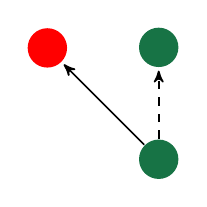
\begin{tikzpicture}[->,>=stealth',shorten >=1pt,auto,node distance=2cm,semithick]
  \tikzstyle{every state}=[draw=none]

  \node[state, fill=darkspringgreen,minimum size=.5cm] 	     (A)                    {};
  \node[state, fill=red,minimum size=.5cm]         (B) [above left of=A] {};
 % \node[state, fill=darkspringgreen,minimum size=.5cm]         (C) [below right of=A] {};
  \node[state, fill=darkspringgreen,minimum size=.5cm] 	     (D) [above =.9cm of A]                   {};

  \path[dashed] (A) edge              (D);
 %           	edge               (C);
  \path[->] (A) edge (B);

      \end{tikzpicture}
          \caption{Primary meristem transitioning to one vegetative meristem and generating one primary meristem.} 
  \end{subfigure}
              \hspace{\fill}
%% PRIMARY MERISTEM PRODUCING INFLORESCENCE MERISTEM
\begin{subfigure}{.25\textwidth}
    \centering
      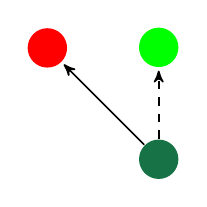
\begin{tikzpicture}[->,>=stealth',shorten >=1pt,auto,node distance=2cm,
                    semithick]

  \node[state, fill = darkspringgreen, draw = none,minimum size=.5cm] (A)                    {};
  \node[state, fill = red, draw = none,minimum size=.5cm]         (B) [above left of=A] {};
 % \node[state, fill = orange, draw = none,minimum size=.5cm]         (C) [above right of=A] {};
  \node[state, fill=green, draw = none,minimum size=.5cm] 	     (C) [above =.9cm of A]                   {};

  \path[dashed] (A) edge              (C);
  \path[->] (A) edge (B);

      \end{tikzpicture}
    \caption{Primary meristem transitioning to one vegetative meristem, and generating one inflorescence meristem.}
      \end{subfigure}
          \hspace{\fill}
%% PRIMARY MERISTEM PRODUCING INFLORESCENCE MERISTEM
      \begin{subfigure}{.25\textwidth}
% stem cell expansion
\centering
% stem cell expansion
      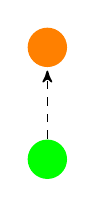
\begin{tikzpicture}[->,>=stealth',shorten >=1pt,auto,node distance=2cm,
                    semithick]

  \node[state, fill = green, draw = none,minimum size=.5cm] (A)                    {};
  \node[state, fill = orange, draw = none,minimum size=.5cm]         (B) [above =.9cm of A] {};
 % \node[state, fill = orange, draw = none,minimum size=.5cm]         (C) [below right of=A] {};

  \path[dashed] (A) edge              (B);
% \path (A) edge		     (B);

      \end{tikzpicture}
    \caption{Inflorescence meristem generating a floral meristem}
  \end{subfigure}
        \caption{Meristem transitions in an unbranched plant with a determinate inflorescence.}
    \label{fig:transitions-unbranched-determinate}
\end{figure}

The table below summarizes the state and control variables in models based on these meristem transitions.
%
\begin{table}[hbt!]
\footnotesize
\begin{tabularx}{\linewidth}{|l|X|}
\hline
\textbf{Term} & \textbf{Description} \\ \hline
 P    & Primary meristems            \\ \hline
 V   &  Vegetative biomass         \\ \hline
 I   &  Inflorescence meristems          \\ \hline
 F   &  Floral meristems          \\ \hline
 $u(t)$   &  The probability that a primary meristem division produces a primary and vegetative meristem (Figure 1A).       \\ \hline
  $1-u(t)$   &  The probability that a primary meristem division produces an inflorescence and a vegetative meristem (Figure 1B).       \\ \hline
   $\beta_1(t)$  &  The per-capita rate of division by primary meristems.     \\ \hline
  $\beta_2(t)$  &  The per-capita rate of division by inflorescence meristems.     \\ \hline
\end{tabularx}
\end{table}

\clearpage
\newpage

\subsection*{Unbranched, determinate case with resource constraint}
We rewrite the optimal control problem to include a state variable inequality constraint, which here is the resource constraint
%
\begin{align}
\max_{u} &  \int_0^T  \log( F(t) ) \dd t & \mbox{ Objective function }   \nonumber \\
\mathrm{subject\ to\ } 
& \dot{P} =  \gamma [\beta_1(t)] [( u(t)) P ] - [\beta_1(t)] [(1 - u(t)) P ] & \mbox{ System of ODEs }   \nonumber \\
& \dot{V} = [\beta_1(t)] [ u(t) P]  + [\beta_1(t)] [(1 - u(t)) P] = \beta_1 [P] \nonumber \\ 
& \dot{I} = [\beta_1(t)] [( 1-u(t) ) P] - [\beta_2(t)] I  \\ 
& \dot{F} = [\beta_2(t)] I  \nonumber \\ 
& P(0) > 0;\ V(0),\ I(0),\ F(0) \geq 0 & \mbox{ Initial conditions}  \nonumber \\
& 0 \le \beta_1(t), \beta_2(t) \le M & \mbox{ Meristem constraint}  \nonumber \\
& 0 \le \beta_1(t) P + \beta_2(t) I \le \alpha V & \mbox{ Resource constraint} \nonumber \\
& 0 \leq u(t) \leq 1 & \mbox{Control constraint} \nonumber 
\end{align}

We write the Hamiltonian as
%
\begin{align}
& H = \log F + \lambda_1 [ - \beta_1 (1-u) P ] + \lambda_2 [ \beta_1 P ]  + \lambda_3 [ \beta_1 (1-u) P - \beta_2 I ] + \lambda_4 [ \beta_2 I ] + \eta [V - (\beta_1 P + \beta_2 I) ]
\end{align}
%
To obtain the switching functions, we take the derivative of the Hamiltonian with respect to each control 
%
\begin{align}
& \frac{\partial H}{\partial u} = (\lambda_1 - \lambda_3) \beta_1 P = 0\ \mathrm{at}\ \beta_1^*, \beta_2^* \\
&\frac{\partial H}{\partial \beta_1} =  (\lambda_3(1-u) - \lambda_1 (1-u) + \lambda_2 - \eta) P = 0\ \mathrm{at}\ u^*, \beta_2^* \\
&\frac{\partial H}{\partial \beta_2} =  (\lambda_4 - \lambda_3 - \eta) I = 0\ \mathrm{at}\ u^*, \beta_1^*
\end{align}
%
The adjoint equations are
%
\begin{align}
&-\frac{\partial H}{\partial P} = \dot{\lambda_1}  = \beta_1 ( \lambda_1 (1-u) - \lambda_2 - \lambda_3 (1-u) + \eta \beta_1 ) \nonumber \\
&-\frac{\partial H}{\partial V} = \dot{\lambda_2}  = - \eta  \nonumber\\
&-\frac{\partial H}{\partial I} = \dot{\lambda_3}  = \beta_2(\eta + \lambda_3-\lambda_4) \nonumber \\
&-\frac{\partial H}{\partial F} = \dot{\lambda_4}  = -\frac{1}{F}  
\end{align}
The transversality condition is
%
\begin{align}
\lambda_1(T) = \lambda_2(T) = \lambda_3(T) = \lambda_4(T) = 0.
\end{align}
%
The complementary slackness condition is 
\begin{align}
& \eta \geq 0,\ \eta [V-(\beta_1 P + \beta_2 I) ] = 0  
\end{align}
% 
From the above equation,  $\eta = 0$ when $V - (\beta_1 P + \beta_2 I) > 0 $ (off the constraint). On the other hand, $\eta > 0$ when $V - (\beta_1 P + \beta_2 I) \leq 0$ (on the constraint).

\hl{When we are not on the boundary, ($V-(\beta_1 P + \beta_2 I)>0$).}

\hl{We do the following on the boundary}
%
\begin{align}
\phi = \frac{ (P(\lambda_3 - \lambda_1) (1-u) + \lambda_2 ) - (I(\lambda_4 - \lambda_3) }{P - I}
\end{align}
%



\end{document}